\chapter{Material and method}
\label{chap:m&m}

\section{Material}
\subsection{Laboratory instruments}
\begin{table}[H]
	\centering
	%\caption{Chemicals used in the master thesis, listed alphabetically according to chemical name, including the chemical's CAS nr., purity/grade, supplier and state.}
	\label{tb:instruments}
	\resizebox{\linewidth}{!}{
	\begin{tabular}{lll}
	\textbf{Instrument} & \textbf{Model} & \textbf{Producer} \\
		\midrule
   Benchtop Flow Cytometer               & BD Accuri$^{TM}$ C6 Plus & BD Biosciences, California, US \\
   Submersible Flow Cytometer            & Cytosub                  & CytoBuoy, Woerden, NL \\
   Coulter Counter                       & Multisizer 4             & Beckman Coulter Inc., California, US \\
   Upright microscope                    & Eclipse Ni-U             & Nikon Corp, Tokyo, JP \\
   Upright microscope                    & Ecliplse 90i             & Nikon Corp, Tokyo, JP\\
   Transmitted/incident light microscope & Labrolux 12              & Leitz, Wetzlar, DE\\
   Benchtop centrifuge                   & Centrifuge 5804 R        & Eppendorf, Hamburg, DE\\
   Counting chamber                      & Bürker                   & Hirschmann-Laborgeräte, Eberstadt, DE \\
   		\bottomrule
	\end{tabular}
}
\end{table}



\subsection{Chemicals}
\begin{table}[H]
	\centering
	%\caption{Chemicals used in the master thesis, listed alphabetically according to chemical name, including the chemical's CAS nr., purity/grade, supplier and state.}
	\label{tb:chemical-list}
	\resizebox{\linewidth}{!}{
	\begin{tabular}{lllll}
	\textbf{Chemicals (abbrv.)} & \textbf{CAS-No.} & \textbf{Purity/grade} & \textbf{Supplier} & \textbf{state} \\
		\midrule
    Calcium chloride dihydrate      & 10035-04-8 & $\geq$ 99.0 \% & Sigma Aldrich & s \\
    Dimethyl sulfoxide              & 67-68-5    & $\geq$ 99.5 \% & Sigma Aldrich & l \\
    D-(+)-Glucose                   & 50-99-7    & $\geq$ 99.5    & Sigma Aldrich & s \\
    \ce{Na2EDTA}$\cdot$\ce{2H2O}    & 6381-92-6  & 98.5-101.5 \%  & Sigma Aldrich & s \\
    Ethanol                         & 64-17-5    & 96 \% vol      & VWR           & l \\
    \ce{Na2HPO4}$\cdot$\ce{2H2O}    & 10028-24-7 & $\geq$ 98.0    & Sigma Aldrich & s \\
    Potassium phosphate monobasic   & 7778-77-0  & $\geq$ 98.0    & Sigma Aldrich & s \\
    Copper(II)sulfate pentahydrate  & 7758-99-8  & $\geq$ 98.0    & Sigma Aldrich & s \\
    Formaldehyde                    & 50-00-0    & 37\% wt        & Sigma Aldrich & l \\
    HEPES                           & 7365-45-9  & $\geq$ 99.5 \% & Sigma Aldrich & s \\
    Magnesium sulfate heptahydrate  & 10034-99-8 & $\geq$ 99.5 \% & Sigma Aldrich & s \\
    Methanol                        & 67-56-1    & $\geq$ 99.9 \% & Sigma Aldrich & l \\
    Potassium chloride              & 7447-40-7  & $\geq$ 99.9 \% & Sigma Aldrich & s \\
    Sodium chloride                 & 7647-14-5  & $\geq$ 99.5 \% & Merck         & s \\
    Trizma\textsuperscript{\textregistered}base & 77-86-1    & ACS reagent    & Merck         & s \\
    TRIS HCl                        & 1185-53-1  & $\geq$ 99.0 \% & Sigma Aldrich & s \\
		\bottomrule
	\end{tabular}
	}
\end{table}


\subsection{Reagents for Flow Cytometry}
\begin{table}[H]
	\centering
	%\caption{Reagents and kits used in the master thesis, listed alphabetically according to product name, including manufacturer, supplier and supplier's catalogue number.}
	\label{tb:reagent-list}
	\resizebox{\linewidth}{!}{
	\begin{tabular}{lllll}
	\textbf{Product name (abbrv.)} & \textbf{Manufacturer} & \textbf{Supplier} & \textbf{Catalogue} & \textbf{Concentration} \\
		\midrule
    TO-PRO$^{TM}$-3 Iodide (642/661) &  InVitrogen$^{TM}$  & Thermo Fisher & T3605 & 1.2 \micro M \\
    Ethidium Homodimer-1 &  InVitrogen$^{TM}$ & Thermo Fisher &  E1169 & 4 \micro L/sample \\
    Apotracker$^{TM}$ Green & BioLegend & Fisher Scientific & 50-207-9934 & 560 nM \\
    Calcein-AM & Invitrogen$^{TM}$ & Thermo Fisher & C1430 & 170 nM \\ 
    CS\&T RUO beads & BD Biosciences & BD Biosciences & 661414 &  4 drops/mL \\
    8-peak validation beads & Spherotech & BD Biosciences & 653144 & 4 drops/mL \\
    6-peak validation beads & Spherotech & BD Biosciences & 653145 & 4 drops/mL \\
		\bottomrule
	\end{tabular}
	}
\end{table}


\subsection{Microscopy kits and reagents}
\begin{table}[H]
	\centering
	%\caption{Reagents and kits used in the master thesis, listed alphabetically according to product name, including manufacturer, supplier and supplier's catalogue number.}
	\label{tb:Microscopy-list}
	\resizebox{\linewidth}{!}{
	\begin{tabular}{llll}
	\textbf{Product name (abbrv.)} & \textbf{Producer} & \textbf{Supplier} & \textbf{Catalogue} \\
		\midrule
    Giemsa's azur eosin methylene blue solution & Merck & Sigma Aldrich & 1.09204.0500 \\
    Hemacolor\textsuperscript{\textregistered} & Sigma Aldrich & Sigma Aldrich & 1.11661 \\
    Eukitt\textsuperscript{\textregistered} Quick-hardening mounting medium & Orsatec GmbH & Sigma Aldrich & 03989 \\
    Type N Immersion Oil for Microscopy & Nikon & ? & MXA20234 \\
    Percoll$^{TM}$ & Cytiva Sweden AB & Sigma Aldrich & GE17-0891-02 \\
		\bottomrule
	\end{tabular}
	}
\end{table}

\subsection{Microscope equipment and software}
\begin{table}[H]
	\centering
	%\caption{Reagents and kits used in the master thesis, listed alphabetically according to product name, including manufacturer, supplier and supplier's catalogue number.}
	\label{tb:Microscope_software-list}
	\resizebox{\linewidth}{!}{
	\begin{tabular}{lll}
	\textbf{Equipment} & \textbf{Model} & \textbf{Producer} \\
		\midrule
   \multicolumn{3}{l}{\textbf{Setup for Nikon 90i:}} \\
   Microscope controller software           & iControl v.2.0.0.3        & Nikon Corp, Tokyo, JP \\          
   Light engine                             & EL6000                    & Leica Microsystems, Wetzlar, DE \\
   Microscope camera                        & DS-Fi1                    & Nikon Corp, Tokyo, JP\\
   DS-Fi1 camera controller                 & DS-U2                     & Nikon Corp, Tokyo, JP \\
   DS-Fi1 digital imaging software          & NIS Elements D v.3.22.15  & Nikon Corp, Tokyo, JP \\
   Microscope camera                        & DS-Fi1c                   & Nikon Corp, Tokyo, JP\\
   DS-Fi1c camera controller                & DS-U3                     & Nikon Corp, Tokyo, JP \\
   DS-Fi1c digital imaging software         & NIS-Elements F v.4.60     & Nikon Corp, Tokyo, JP \\
   Flat top microscope stage                & Proscan H101/2            & Prior Scientific, Cambridge, UK \\
   Microscope stage encoder                 & Lie5 1P N2KV              & Numerik Jena, Jena, GE \\
   Microscope stage controller              & Proscan II                & Prior Scientific, Cambridge, UK\\
   Filtercube                               & Brightline\textsuperscript{\textregistered} Led-Cy5-A  & Semrock \\
   Filtercube                               & B-2A                      & Nikon Corp, Tokyo, JP \\
   Stage micrometer cal. slide              & 2 mm, 0.01 mm interval    & Leitz, Wetzlar, DE \\
   Objective lens                           & Plan Apo 20X/0.75         & Nikon Corp, Tokyo, JP \\
   Objective lens                           & Plan Apo 60XA/1.40 Oil    & Nikon Corp, Tokyo, JP \\
   Objective lens                           & Plan Apo VC 100X/1.40 Oil & Nikon Corp, Tokyo, JP\\
   
   && \\
   \multicolumn{3}{l}{\textbf{Setup for Nikon Ni-U:}} \\
   Light engine                             & Sola SM II 365            & Lumencor Ink., Greenbrier, US \\
   CMOS camera                              & MC170HD                   & Leica Microsystems, Wetzlar, DE \\
   Microscope camera                        & 4KHDMI                    & DeltaPix, Smorum, DK\\
   Objective lens (Nikon Ni-U)              & Plan Fluor 40X/0.75       & Nikon Corp, Tokyo, JP \\
   Objective lens (Nikon Ni-U)              & Plan Fluor 100X/1.30      & Nikon Corp, Tokyo, JP \\
		\bottomrule
	\end{tabular}
	}
\end{table}




\subsection{Buffers and solutions}
\begin{table}[H]
	\centering
	\label{tb:buffers}
	\resizebox{\linewidth}{!}{
	\begin{tabular}{ll}
	\textbf{Buffer} & \textbf{Composition} \\
		\midrule
    MAS                   &  375.6 mM \ce{NaCl}, 28.97 mM Citric Acid$\cdot$3Na$\cdot$2\ce{H2O}, 113.8 mM D-Glucose, \\ 
                          & 2.6 mM Citric Acid$\cdot$\ce{H2O}, 11.5 mM \ce{Na2EDTA}$\cdot$\ce{2H2O}, pH=7.0, 0.2 \micro m filtered \\
    Anticoagulant buffer  & 55.5 mM D-glucose, 171.1 mM NaCl, 13.4 mM \ce{Na2EDTA}$\cdot$\ce{2H2O}, \\
                          & 0.05 M TRIS/HCl, pH=7.6, 0.2 \micro m filtered \\ 
    PBS                                  & 136.9 mM \ce{NaCl}, 2.7 mM \ce{KCl}, 10.1 mM \ce{Na2HPO4}, 1.8 mM \ce{KH2PO4} \\
    Sorensen Buffer       & 66.7 mM \ce{KH2PO4}, 66.7 mM \ce{Na2HPO4}$\cdot$\ce{2H2O}, pH=6.8, 0.2 \micro m filtered \\
    MPSS    &  470 mM \ce{NaCl}, 10 mM \ce{KCl}, 10 mM \ce{CaCl2}, 10 mM HEPES \\
                          & 47.7 mM \ce{MgSO4}, pH=7.41, 0.2 \micro m filtered \\
    Tris Buffered Saline  & 44.5 mM Trizma\textsuperscript{\textregistered}base, 5.5 mM TRIS-HCl, 450 mM \ce{NaCl}, pH=7.00 \\
		\bottomrule
	\end{tabular}
	}
\end{table}


\section{Method development}
This section describes in detail the work and experiments that were performed in the development of a hybrid flow cytometry- and microscopy-based version of The Mussel Micronucleus Cytome Assay by Bolognesi and Fenech (2012). The finalized assay is presented in it's entirety in the method section, in the context of it's application to test the potential genotoxic and cytotoxic effects of aged \ce{TiO2} and Ag \acrshort{ENPs}. The results from this section is presented in the Results chapter (\ref{section:Results_Method_Development}), and the reader can benefit from a read through that section before continuing with the method section and the main results (4.2).

Include some technical stuff? E.g., unless stated otherwise, 10.000 events were acquired from each sample with 36 uL/min and 16 \micro L core size. 80.000 FSH-H was used as the only threshold, and doublet haemocytes were gated out of analysis with a FSH-H vs FSC-A singlets gate.

\subsection{Haemolymph sampling technique}
\label{subsection:haemolymph sampling technique}
To minimize the possibility of contaminating hemolymph samples during extraction, a simple and time-effective sampling technique adapted from the nonlethal technique of Gustafson et al., 2005 was used. "Blind" methods of withdrawal through a notch in the posterior dorsal shell or through the exhalant syphon frequently resulted in considerable contamination with debris from the pallial fluid. Therefore, the hemolymph sampling technique employed was centered around achieving good visual contact with the posterior adductor muscle and the position of the needle within the muscle during hemolymph withdrawal, and was mainly constricted by the requirement of an intact digestive gland.

The digestive gland is located dorsally (towards the hinge), slightly off-center towards the anterior end of the shell (Eggermont, 2020). In order to access and see the posterior adductor muscle while staying clear of the digestive gland, the valves were prised apart ventrally by gently forcing a tissue forceps between the valves midway of the mussel's length, or slightly posterior of the byssal mass (Figure \ref{fig:Hemolymph_sampling_illustration}a). When the pallial cavity opened, pallial fluid (seawater) was drained away from the posterior adductor muscle by positioning the mussel's umbo on a paper tissue for 15-30 seconds. Since the posterior adductor muscle is oblong in the anteroposterior direction, penetrating the muscle from the posterior end pointing straight anteriorly gave the operator better margins to avoid piercing the muscle.

To create a free path to the muscle from the posterior direction, the connecting mantle immediately surrounding the exhalant syphon were cut with a scalpel (Figure \ref{fig:Hemolymph_sampling_illustration}b and d), holding the blunt spine of the blade facing the posterior adductor muscle. Thus, when illuminating the pallial cavity from above with the ventral aspect facing upwards, the operator was able to supervise the position of the needle inside the posterior adductor muscle sinus through the slightly transparent muscle fibers, as seen in Figure \ref{fig:Hemolymph_sampling_illustration}c.

\begin{figure}[H]
    \centering
    \begin{subfigure}[b]{.45\textwidth}
        \centering
        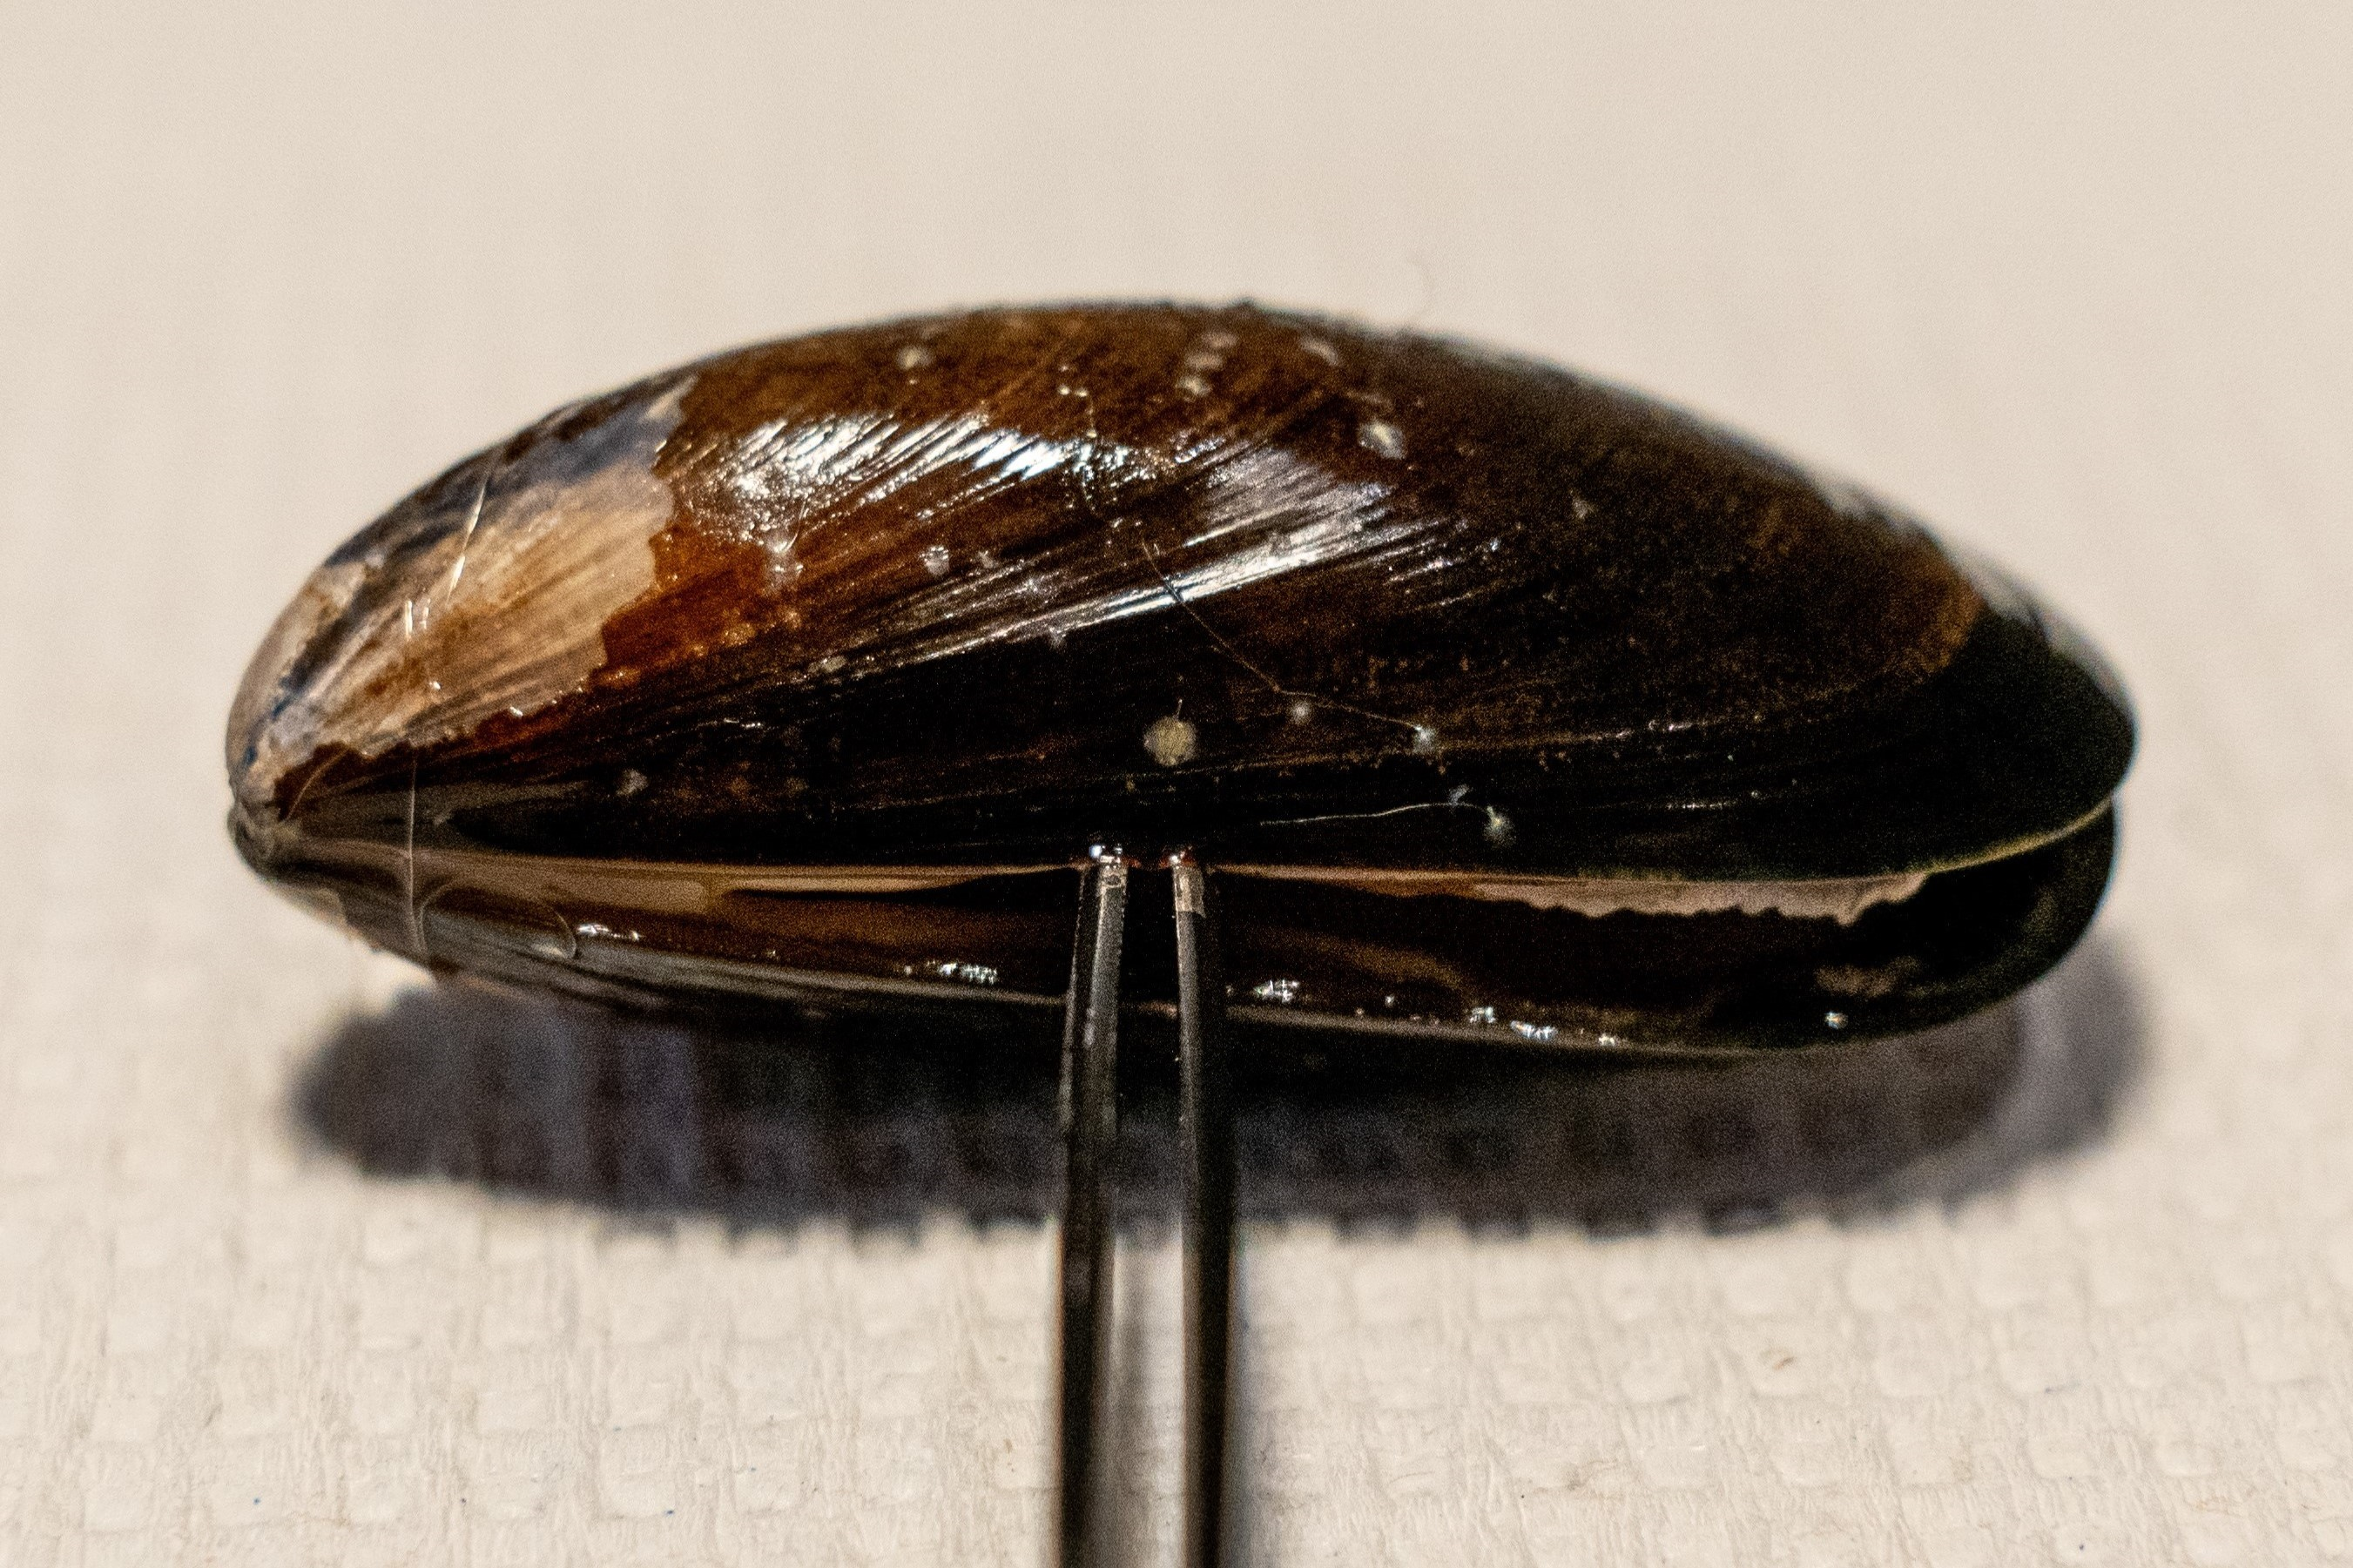
\includegraphics[width=\textwidth]{figures/Sampling technique/forceps square color.jpg}
        \caption{Placement of forceps between valves on the ventral side of the mussel.}
        \label{sfig:a}
    \end{subfigure}
    \hfill
    \begin{subfigure}[b]{.45\textwidth}
        \centering
        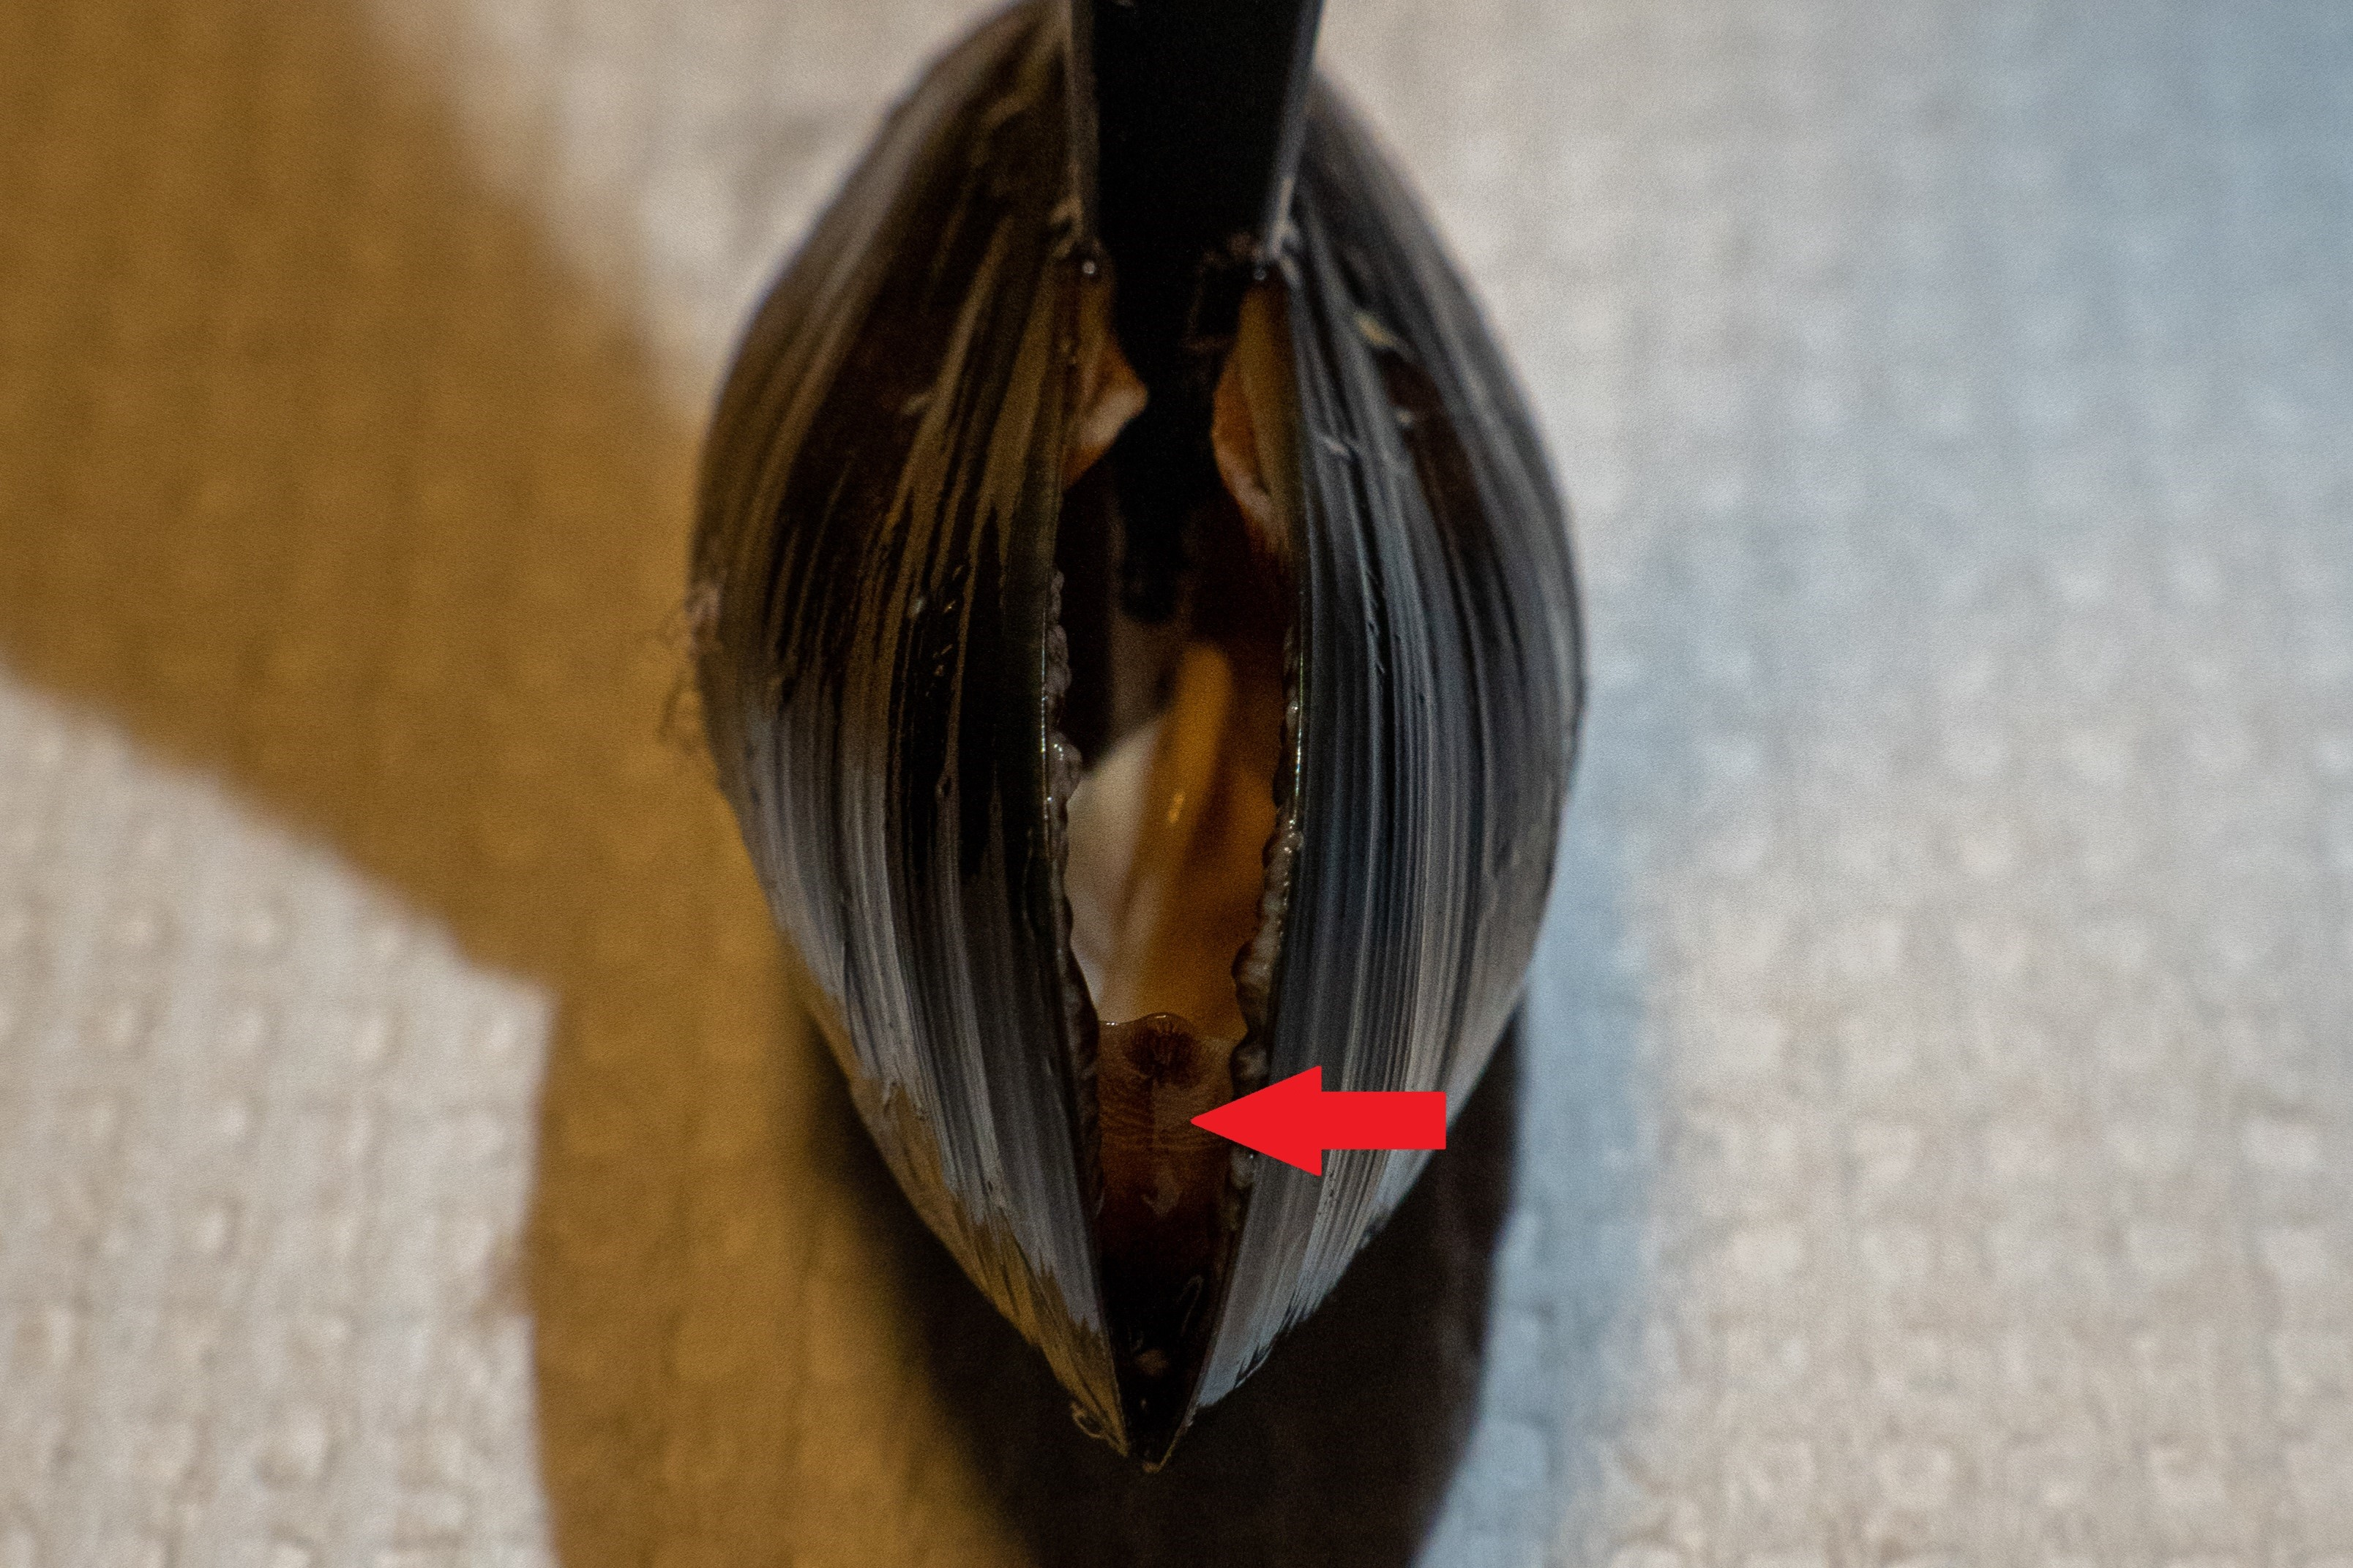
\includegraphics[width=\textwidth]{figures/Sampling technique/uncut color 3495.jpg}
        \caption{Posterior aspect of mussel with the connecting mantle (red arrow) intact.}
        \label{sfig:b}
    \end{subfigure}
    \newline
    \begin{subfigure}[b]{.45\textwidth}
        \centering
        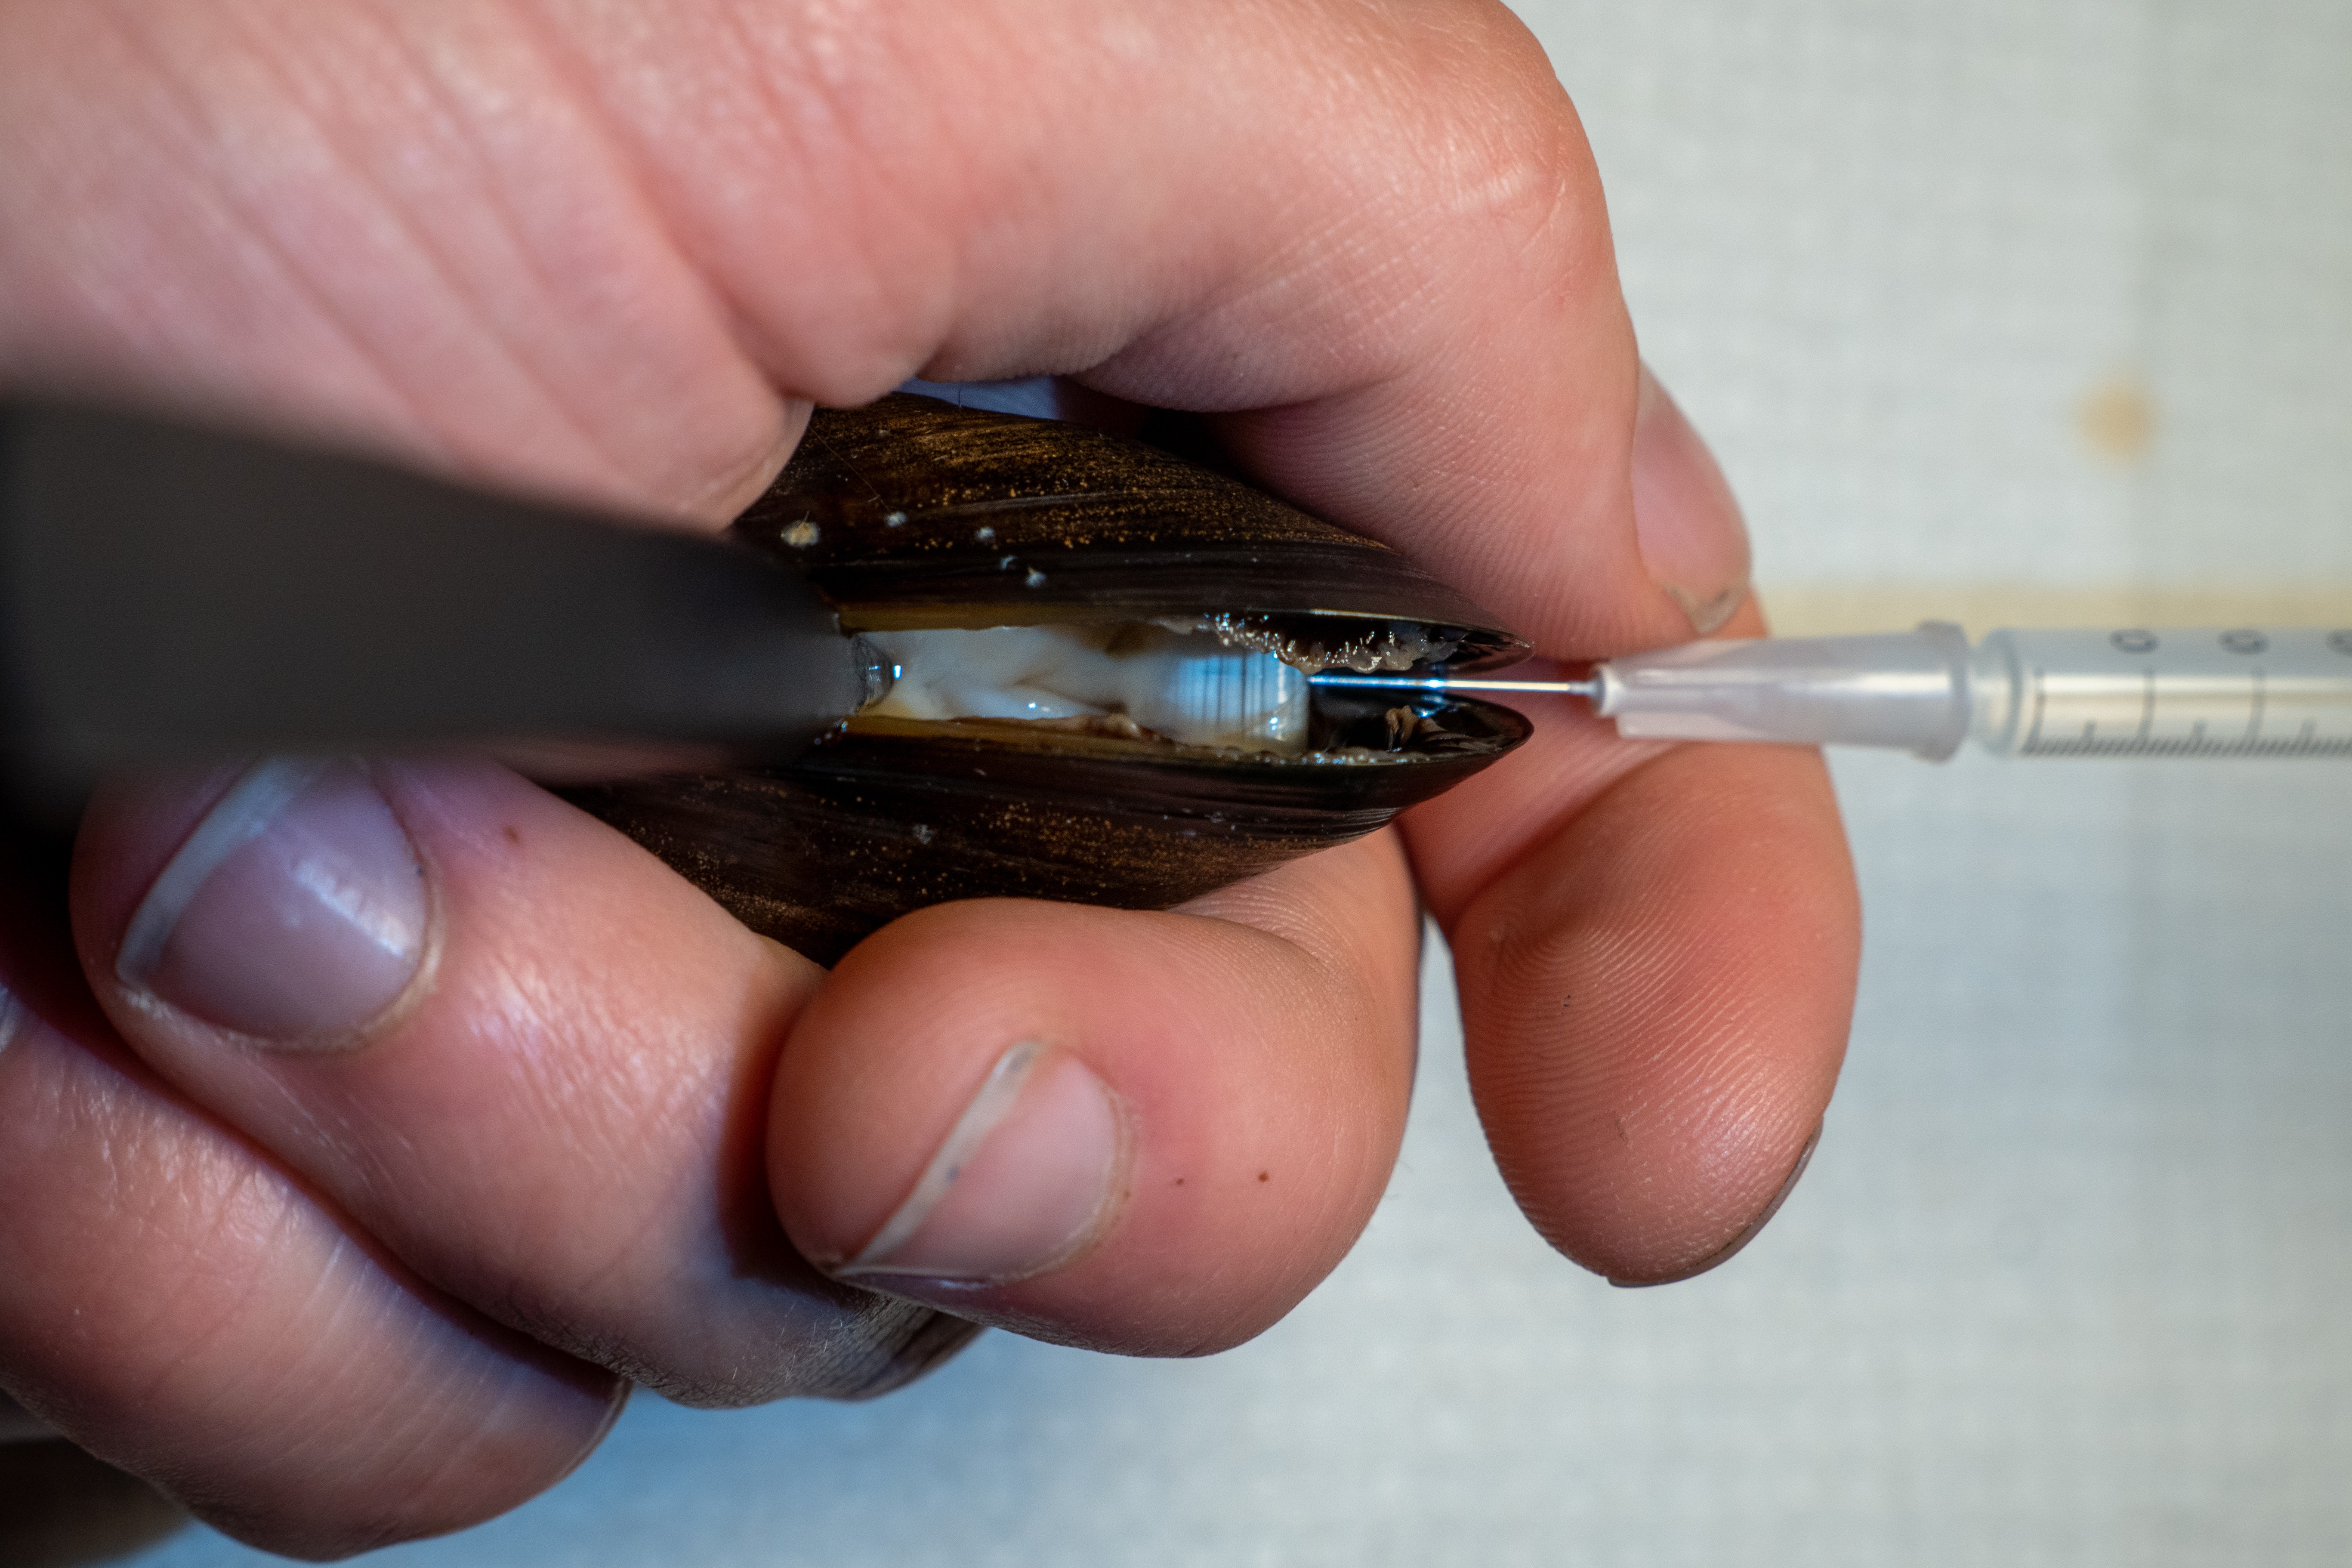
\includegraphics[width=\textwidth]{figures/Sampling technique/hands colors centered.jpg}
        \caption{The mussel grip and needle alignment employed, seen from the operators perspective.}
        \label{sfig:c}
    \end{subfigure}
    \hfill
    \begin{subfigure}[b]{.45\textwidth}
        \centering
        \includegraphics[width=\textwidth]{figures/Sampling technique/possible match.jpg}
        \caption{Mussel with visible posterior adductor muscle (red arrow) where the mantel was cut.}
        \label{sfig:d}
    \end{subfigure}
    \caption{An illustration of the method employed to extract hemolymph from the posterior adductor muscle of M. edulis in order to avoid off-target withdrawal of pallial fluid or spermatozoa. The images were captured using a Sony A6400 mirrorless digital camera with a Tamron 17-70mm F/2.8 lens, and were edited with Adobe\textsuperscript{\textregistered} Lightroom Classic 12.0 image editing software.}
    \label{fig:Hemolymph_sampling_illustration}
\end{figure}

For this work, 1.0 mL syringes equipped with sterile 23 gauge hypodermic needles were used. Hemolymph samples were gently withdrawn at an approximate rate of 1.0 mL/min, in order to prevent the negative pressure inside the muscle from drawing in pallial fluid between the muscle fibers. The mussels were placed in the palm of the operator's non-dominant arm, 3$^{rd}$-5$^{th}$ digits firmly gripping the mussel, 1$^{th}$ and 2$^{nd}$ digits keeping the syringe steady in the anteroposterior direction, while the dominant hand were used to withdraw the syringe plunger.

\subsection{Selection of haemocyte medium for flow cytometry assays}
The haemocytes of \emph{M. edulis} have a tendency to form aggregates upon mechanical stress, e.g. when the hemolymph is withdrawn through a thin syringe needle. Since accurate flow cytometric analyses rely on single-cell measurements, there was a need to minimize haemocyte aggregation during staining procedures, until the samples could by analyzed on the flow cytometer. In the literature, several authors have dealt with this challenge by aspirating hemolymph samples directly into slightly acidic \acrshort{edta}-containing solutions buffered by citric acid (\cite{Söderhall1983, Bachere1988, LeFoll2010}). Since haemocyte aggregation is a Ca$^{2+}$-dependent process (\cite{Torreilles1999, Chen1995}), withdrawal of hemolymph into buffers containing divalent metal-ion chelators effectively slows the rate of haemocyte aggregation, allthough it does not inhibit aggregation completely (\cite{Chen1995}). Another frequently reported method is to dilute the hemolymph in cold filtered seawater (\acrshort{fsw}), while keeping the samples on ice prior to analysis. 

In search for the most effective method for this work, hemolymph samples were withdrawn into syringes pre-filled with a number of different "anticoagulant" or "antiaggregative" buffers (1:1) reported in the literature. The degree of aggregation was initially evaluated by inspecting hemolymph smears prepared following the method of Bolognesi and Fenech (2012) under 10x magnification. After preliminary testing, the most promising buffers encountered where the Modified Alsever's Solution (\acrshort{mas}, pH=6.2), and the similar Anticoagulant Buffer (\acrshort{acb}, pH=7.6) with \acrshort{edta} reported by \cite{Pipe1997}. Since the use of \acrshort{edta} (\acrshort{mas} and \acrshort{acb}), acidic pH (\acrshort{mas}) or keeping samples on ice (\acrshort{fsw}) might introduce inconveniences related to staining procedures, extra handling requirements and possibly impairing haemocyte viability, two experiments were devised in order to test their relative effects on haemocyte aggregation and viability - under the conditions intended for our flow cytometric analysis. Thereby, a cost-effect assessment could be carried out to arrive at the most suitable buffer for this work.

\subsubsection{Haemocyte aggregation}
An experiment was seeded from the observation that \acrshort{fcm} singlet haemocyte counts tended to decrease over time from hemolymph withdrawal, and were based on the assumption that aggregation was the main driving factor. The proportion of aggregated haemocytes in a sample at a given time could therefore be retraced from the initial haemocyte count when performing several counts of the same sample over time. Since the difference in density between buffers would be negligible, the sedimentation rates would be independent of the haemocyte medium. Any observed differences would thus be caused by differences in the buffers' ability to inhibit aggregation.

500 \micro L hemolymph was withdrawn from 24 individual mussels into syringes prefilled with either 500 \micro L \acrshort{mas} (RT, n=8), \acrshort{acb} (RT, n=8) or cold Marine Physiological Saline Solution (\acrshort{mpss}, \SI{4}{\celsius}, n=8). Tris-buffered \acrshort{mpss} (pH=7.4) was used as a proxy for \acrshort{fsw}, such that pH and osmolarity could be controlled. The diluted hemolymph was transferred to 12$\times$75 mm polystyrene tubes and the initial haemocyte count were determined by acquiring 20 \micro L sample on the flow cytometer immediately thereafter. Each sample was run with identical acquisition and fluidics settings (see table \ref{tb:FCM_settings}), and the cells were gated on by a singlet inclusion gate (FSC-A vs. FSC-H) and a haemocyte gate (FSC-A v. SSC-A, see gating strategy). To account for any extra aggregation occurring from gentle mixing with flow cytometry reagents in the planned assay, each sample was gently pipetted up and down four times following the initial count. The second count were performed precisely 15 minutes later to mimic the incubation periods of our flow cytometry reagents. Three more singlet haemocyte counts where acquired from each sample at 30, 45 and 60 minutes post-withdrawal, to discern the buffers' ability to prevent aggregation during longer incubation periods. Samples withdrawn into \acrshort{mpss} were kept on ice between each singlet haemocyte count.

\subsubsection{Mixed logistic regression of the proportion of aggregated haemocytes}
The dataset consisted of 107 observations ($y_{ij}, t_{ij}$) from 24 individual mussels ($i$), $i = 1,...,n_{i}$, where $y_{ij}$ denotes the proportion of aggregated haemocytes from mussel $i$ at timepoint $t_{ij}$, $j = 1,...,n_{j}$, and $j$ represents repeated measurements of mussel $i$ at $t = (0, 60]$ minutes post-withdrawal. If we let $N_{t0}$ represent the initial haemocyte count of mussel $i$ at $t \approx 0$, the proportion of aggregated haemocyte at time $t_{ij}$ was calculated according to (\ref{eq: proportion_agg}):

\begin{equation}
    \label{eq: proportion_agg}
    y_{ij} = \dfrac{N_{t0} - N_{ij}}{(N_{t0} - N_{ij}) + N_{ij}} = \dfrac{N_{t0} - N_{ij}}{N_{t0}}
\end{equation}

\noindent where $N_{ij}$ denotes the hemocyte count of mussel $i$ at time $t_{ij}$.

The buffers' ability to inhibit haemocyte aggregation was tested statistically by mixed effects logistic regression, such that the within-individual correlation could be modelled as random effects to account for repeated measurements. The proportions were modelled as a function of log time, with buffer as a categorical explanatory variable. The mixed logistic regression model was fitted by maximum likelihood (Laplace approximation) using the \emph{glmer} function of the R package \emph{lme4} (\cite{lme4}), with a "binomial" error distribution and "logit" link function, as shown in Code listing 3.1. However, instead fitting the model with the calculated proportions ($y_{ij}$), the response variable was formatted as a two-column matrix of aggregated and singlet haemocyte counts, for the response to be weighted by $N_{t0}$. The format of the response matrix is shown in (\ref{eq:agg_free_matrix}).

\begin{lstlisting}[language=R, caption = {The R source code run to fit the logistic proportion aggregation model.}]
model = glmer(data = df, formula = y ~ log(t)*Buffer + (log(t)|ID),
                 family = binomial(link = "logit"))
\end{lstlisting}

\begin{equation}
    \label{eq:agg_free_matrix}
    y_{i} := \begin{pmatrix}
     M_{1} \\
     \vdots \\
     M_{i} \\
     \vdots \\
     M_{n_{i}} \\
    \end{pmatrix}
    , \; \; \; \; M_{i} \: = \:
    \begin{pmatrix}
      N_{t0} - N_{i1}     &  N_{t0} \\
      \vdots              &  \vdots \\
      N_{t0} - N_{ij}     &  N_{t0} \\
      \vdots              & \vdots \\
      N_{t0} - N_{in_{j}} &  N_{t0} \\      
    \end{pmatrix}
\end{equation}

The factor levels of the categorical explanatory variable was defined as dummy variables (see equation \ref{eq:dummy_variables}), where the \acrshort{mpss} buffer was set as reference level. Thus, the fitted proportion of aggregated haemocytes ($y_{ij}$) in a sample from mussel \emph{i} = [1, 24] at time $t_{ij}$, \emph{j} = (0, 60], can be written out on \emph{logit} scale as in (\ref{eq:logit}), where $\alpha_{1} \: + \: \beta_{1}log(t_{ij})$ is the linear predictor of the reference level, $\alpha_{2}$ and $\alpha_{3}$ represents the difference in y-intercept for the \acrshort{acb} and \acrshort{mas} buffers, $\beta_{2}$ and $\beta_{3}$ represents the differences in slopes, while $\gamma_{0i}$ and $\gamma_{1i}$ represents the individual-specific deviation from the population intercept and slope, respectively. The linear predictors relate to the log proportions according to (\ref{eq:linear_predictors}), where the dummy variables $D_{2}$ and $D_{3}$ have been solved according to (\ref{eq:dummy_variables}).

\begin{equation}
    \label{eq:dummy_variables}
D_{2} =\begin{cases}
      1, & \text{ACB}\\
      0, & \text{not ACB},
    \end{cases}
    \quad
D_{3} =\begin{cases}
      1, & \text{MAS}\\
      0, & \text{not MAS}
    \end{cases}
\end{equation}

\begin{equation}
\label{eq:logit}
y_{ij} = \dfrac{1}{1 + e^{-(\alpha_{1} \: + \: \beta_{1} log(t_{ij}) \: + \: D_{2}(\alpha_{2} + \beta_{2}log(t_{ij})) \: + \:  D_{3}(\alpha_{3} + \beta_{3}log(t_{ij})) \: + \: \gamma_{0i} \: + \: \gamma_{1i}log(t_{ij}))}}
\end{equation}

\begin{equation}
    \label{eq:linear_predictors}
    \resizebox{\linewidth}{!}{$
    log\dfrac{P(y_{ij} = 1 \mid t_{ij}, \gamma_{0i}, \gamma_{1i})}{P(y_{ij} = 0 \mid t_{ij}, \gamma_{0i}, \gamma_{1i})} = \begin{cases}
        \alpha_{1} + \gamma_{0i} + (\beta_{1} + \gamma_{1i})log(t_{ij}), & i \: \text{in MPSS group}, \\
        \alpha_{1} + \alpha_{2} + \gamma_{0i} + (\beta_{1} + \beta_{2} + \gamma_{1i})log(t_{ij}), & i \: \text{in ACB group}, \\
        \alpha_{1} + \alpha_{3} + \gamma_{0i} + (\beta_{1} + \beta_{3} + \gamma_{1i})log(t_{ij}), & i \: \text{in MAS group} \\
    \end{cases}
    $}
\end{equation}

Since generalized linear mixed models (\acrshort{glmms}) do not allow for a marginal interpretation of coefficients, the group-averaged proportions of aggregated haemocytes after 15 minutes post-withdrawal were compared by conventional two-sample t-tests. This timepoint was chosen specifically, since the required incubation with flow cytometric viability dyes would most likely not surpass 15 minutes.

\subsubsection{Haemocyte viability}
One of the aims of this project was to count the number of necrotic haemocytes present in the hemolymph of \emph{M. edulis} by means of flow cytometry. Since the mussels were to be exposed to \ce{TiO2} and Ag nanoparticles \emph{in vivo} for 21 days, the targeted endpoint would be the number of necrotic haemocytes circulating in their hemolymph at the timepoint just before hemolymph extraction on day 22. Any acute effects on viability arising from the hemolymph extraction itself, or during incubation with the viability stains between extraction and count, would serve to obscure the potential \emph{in vivo} effect of the nanoparticles. When choosing a suitable anticoagulant buffer for the purpose of this measurement, it was therefore essential to make sure that the buffer itself did not interfere with the targeted endpoint.

To test wether the \acrshort{edta}-containing buffers had any effects on haemocyte viability in the 15 minute time window required for staining, 500 \micro L hemolymph was withdrawn from 24 individual mussels into syringes prefilled with either 500 \micro L \acrshort{mas} (n=8) or \acrshort{acb} (n=8). Hemolymph from the last eight mussels were withdrawn into cold \acrshort{mpss} and kept on ice as negative \acrshort{edta}-controls. The diluted hemolymph were transferred to 12$\times$75 mm polystyrene tubes, were they were stored for 15 minutes before staining 300 \micro L subsamples with 1.0 \micro L \acrshort{calceinam} (50 \micro M) and 3.6 \micro L TO-PRO$^{TM}$-3 Iodide (100 \micro M) dissolved in \acrshort{dmso}. The samples were incubated in darkness for 15 minutes, before 10.000 haemocyte events were recorded on the flow cytometer without washing.

488 nm-exited green fluorescence from hydrolyzed Calcein were recorded on the FL1 detector with a 533/15 nm filter, while the 640 nm-exited far red fluorescence from DNA-bound TO-PRO$^{TM}$-3 Iodide were recorded on the FL4 detector with a 675/25 nm filter. The events were gated according to the gating strategy in figure (ref figure), obtaining counts of live (Calcein$^{+}$ToPro3$^{-}$), necrotic (Calcein$^{-}$ToPro3$^{+}$) and doubly stained (Calcein$^{+}$ToPro3$^{+}$) haemocytes, as well as non-cellular particles (Calcein$^{-}$ToPro3$^{-}$) and a total count. In this particular experiment the doubly stained haemocytes were counted as necrotic, as newly damaged or lysed haemocytes might still retain a degree of non-specific esterase activity. Hence, the percentage of necrotic haemocytes were calculated according to equation \ref{eq:necrotic hemocytes}.

\begin{equation}
    \label{eq:necrotic hemocytes}
    \text{Necrotic haemocytes (\%)} = \dfrac{n_{Calcein^{-}ToPro3^{+}} + n_{Calcein^{+}ToPro3^{+}}}{n_{total} - n_{Calcein^{-}ToPro3^{-}}} \times 100
\end{equation}

The 700 \micro L remaining of each hemolymph sample were stored for another 2 and 20 hours, and the same staining and flow cytometric measurements were repeated at these timepoints. Because of considerable aggregation and sedimentation of haemocytes in \acrshort{mpss} after 2 and 20 hours, and those kept in \acrshort{mas} and \acrshort{acb} for 20 hours, the haemocytes in these samples were resuspended with a wide bore pipette before the second and third rounds of staining.

\subsubsection{Haemocyte viability: Statistical analysis}
The mean percentage of necrotic haemocytes in \acrshort{mpss}, \acrshort{acb} and \acrshort{mas} were compared by one-tailed two-sample t-tests at the three different timepoints. Since the group variances ($s^{2}$) differed by more than a factor of 2 at the last timepoint, these comparisons were bade by Welch two-sample t-tests. Paired t-tests were used to assess wether the percentages of necrotic haemocytes increased with incubation time within each group. 

\subsection{Cytologic characterization of haemocyte subpopulations}
\label{subsection:morph}
For the purpose of characterizing and imaging the different haemocyte cell types of \emph{M. edulis} in a non-spread state, samples were withdrawn into an equal volume of ice-cold \acrshort{mpss} and transferred directly onto glass slides. The glass slides were kept in a humid chamber for up to 5 minutes before cells were fixed in ice cold methanol (5$\times$ 1 sec dips). This assured haemocyte attachment, but circumvented the profound morphological changes accompanied by the haemocytes’ process of spreading. Slides were stained with the Hemacolor\textsuperscript{\textregistered} kit according to the manufacturer’s recommendations, air dried, mounted with Eukitt\textsuperscript{\textregistered} and coverslipped. Stained haemocytes were examined and imaged under brightfield illumination on a Nikon Eclipse 90i upright microscope with a 100$\times$/1.40 oil immersion objective and a Nikon DS-Fi1 microscope camera.

Haemocyte morphology was primarily characterized on the basis of cytoplasmic staining, granularity (granule size, abundance and staining affinities), nuclear:cytoplasmic (N:C) ratio, size and shape. Since Le Foll and colleagues (2010) reported that the motile properties of the different haemocyte subpopulations of \emph{M. edulis} could be used as an additional functional criteria for their characterization, the spreading behavior of the different cell types were included to expand on the morphological characteristics. This comprehended a description of the typical haemocyte shapes and motile structures that were observable under differential interference contrast illumination in spread haemocytes. The preparation of slides with spread haemocytes followed a methodology similar to that of the non-spread haemocytes, but the humid chamber incubation periods prior to fixation and staining were extended (15-30 min). Microscopic fields were examined through a 60$\times$/1.40 oil immersion objective under DIC illumination.

\subsection{Determination of cell diameters}
\label{subsection:CytCar}
To establish wether haemocyte subpopulations differed with regard to size across a larger population of adult mussels, the cell diameters of 100 haemocytes were ascertained in haemolymph smears from 20 individual mussels (n=2000). Since the rate and degree of haemocyte spreading could be inherently different among cell types, all spreading was effectively impeded by collecting haemolymph samples into an equal volume of 5\% formaldehyde in \acrshort{mpss}. The fixation was continued for one hour in suspension, before cells were pelleted by centrifugation (250G, 15 min, \SI{10}{\celsius}) and resuspended in 100 \micro L 0.75 \% eosin in Sorensen Buffer. After staining for 5 minutes, 1 mL 3\% Wright’s-Giemsa was added and the staining was continued for an additional 15 minutes. Stained haemocytes were pelleted by centrifugation (180G, 12 min, \SI{10}{\celsius}), resuspended in 100-200 \micro L Sorensen Buffer and transferred onto glass slides. The slides were air-dried in a fume hood until the smears were completely dry and transparent, before they were mounted with Eukitt\textsuperscript{\textregistered} and coverslipped.

The slides were placed on the stage of a Nikon Eclipse 80i upright microscope, and 10-20 microscopic fields from each smear was photographed under DIC illumination with a $\times$60 oil immersion objective. Cell diameter measurements were performed digitally with ImageJ (NIH, Bethesda, Maryland, US), using the \emph{Straight line tool} of this image processing software. The actual size of the magnified haemocytes were determined by calibrating the software's pixel/\micro m scale with a stage micrometer calibration slide (Leitz Wetzlar, Buffalo, DE), photographed with the same equipment and image resolution as the haemolymph smears. When haemocyte outlines deviated from an approximate spherical shape, the diameter was estimated as the average length of the long and short axes, after Burkhard et al. (2009). The measurements were performed as differential counts, such that the number of measurements of each cell type reflected their average relative proportions (\%) across all 20 mussels.

\subsection{Flow cytometric characterization of haemocyte subpopulations by light-scatter measurements}
Throughout the methodological and experimental work that was done in relation to this project, more than 500 adult mussels were samples for haemolymph, and the majority of these samples were run as suspensions of living haemocytes on the BD Accuri C6 Plus Flow Cytometer. The purposes of these measurements varied to a large extent, but the samples were invariably examined as bivariate plots of Forward Scatter (FSC) vs. Side Scatter light (\acrshort{ssc}) at some point in the analyses. These investigations revealed a substantial amount of variation between individual mussels in terms of the relative proportions of their haemocyte subpopulations and their separation according to FSC vs. \acrshort{ssc}.

A quantitative flow cytometric characterization of the haemocyte subpopulations of \emph{M. edulis} can be found in Le Foll et al. (2010), who utilized a flow cytometer equipped with a Coulter-type electronic cell-volume analyzer to characterize haemocytes in terms of cell diameter (\micro M) vs. \acrshort{ssc}. Instead of repeating this endeavor with relative units of \acrshort{fsc}, the scope of the current flow cytometric characterization was to present the typical light-scatter profile of adult mussels, while representing the observed variation with a few examples of extreme observations. The haemolymph samples were withdrawn into an equal volume of \acrshort{acb} according to the technique described in section \ref{subsection:haemolymph sampling technique}, and were analyzed on the flow cytometer directly thereafter.

\subsection{Relating cytologically defined cell types to light-scatter profiles}
As mentioned in theory section \ref{subsection:haemocyte_classification}, the use of flow cytometers with cell sorting capabilities can simplify the process of verifying a classification derived from flow cytometric measurements. However, since the BD Accuri C6 Plus is not equipped with a cell sorter, other measures were taken to relate the cytologically defined cell types in section \ref{subsection:Results_cytchar} to the subpopulations defined by flow cytometry in section \ref{subsection:Results_FlowChar}.

Cell sorters facilitate visual inspections of cells with known measured characteristics following a flow cytometric measurement. This workflow can be reversed if the cells are sorted by other means prior to flow cytometric acquisition. This section describes how pools of Giemsa-stained haemocytes were separated by isopycnic centrifugation, and how the isolated cell fractions were characterized by flow cytometry and microscopy thereafter. Subsequently, the flow cytometric "separation" of haemocytes according to eosin fluorescence is described.

\subsubsection{Isopycnic centrifugation}
Formaldehyde-fixed haemocytes were separated on discontinuous Percoll gradients according to the protocol by Friebel and Renwrantz (1995), with minor modifications. The separation was performed in duplicate with pooled haemocytes from a total of six adult mussels (shell length 58$\pm{12}$ mm). For both gradients, the haemolymph of three individual mussels (1.5-2.0 mL/mussel) were withdrawn into an equal volume of 5\% formaldehyde in \acrshort{mpss}, wherein the haemocytes were fixed for one hour after pooling. The fixed haemocytes were stained with 0.75 \% Eosin and 3 \% Giemsa according to the procedure in section~\ref{subsection:CytCar}. After pelleting, stained haemocytes were resuspended in Tris-Buffered Saline (\acrshort{tbs}, 900 mOsm) to an approximate concentration of $9\times10^{6}$ cells/mL, before layering 2 mL suspension on top of both gradients. Discontinuous Percoll gradients consisted of 15\%, 33\%, 38\%, 43\% and 90\% Percoll stock in \acrshort{tbs} (vol/vol), and were constructed by carefully layering 2 mL of each Percoll concentration in 15 mL Falcon centrifuge tubes with conical bottoms (Corning, New York, US).

The centrifugation was started at 120G for 10 minutes (\SI{4}{\celsius}), followed by 40 minutes at 2500G. An Eppendorf 5804 R benchtop centrifuge equipped with an A-4-44 swing-bucket rotor was employed for the separation, with the brake ramp set to 1. The separated cell fractions were collected into syringes by puncturing the tubes below the gradient interfaces with 23G hypodermic needles. According to a protocol by Bachére and Grizel (1988), the Percoll was eliminated from the 43/90\% and 38/43\% fractions by two consecutive dilutions in \acrshort{tbs} (1:7) and a 10\% sucrose cushions (1:1) before centrifugation (800G, 15 min, \SI{4}{\celsius}). Haemocytes collected from the 15/33\% interface were centrifuged directly after a seven-fold dilution in \acrshort{tbs} (800G, 15 min, \SI{4}{\celsius}).

The pelleted cell fractions were resuspended in Sorensen buffer and divided into two aliquots; one aliquot were used to prepare smears according to the procedure in section \ref{subsection:CytCar}, while the remaining aliquots were further diluted in 1 mL Sorensen buffer for flow cytometric characterization. A total of 10.000 events were acquired from each cell fraction on the flow cytometer (36 \micro L flow rate, 16 \micro m core size), in addition to 30.000 events from both pools that were set aside prior to centrifugation. The relative proportion (\%) of cell types in each fraction were ascertained by performing 1000-cell differential counts.

\subsubsection{Identification of eosinophilic granulocytes by SSC and eosin fluorescence}
Since Eosin is fluorescent in the green/yellow spectrum (\acrshort{exmax}/\acrshort{emmax}: 517/543 nm) (\cite{Koegle2020}), blue laser-exited fluorescence from this anionic dye can be collected on the FL1 detector (518-548 nm) of the BD Accuri C6 Plus flow cytometer (BD Biosciences, California, US). If the haemocytes of \emph{M. edulis} are permeabilized and stained with eosin prior to flow cytometric analysis, the fluorescent signal from Eosin can in theory be used to identify eosinophilic granulocytes on \acrshort{fsc} vs. \acrshort{ssc} dotplots by backgating.

This approach was attempted by Le Foll an colleagues (2010), who detached spread haemocytes stained by eosin with an \acrshort{edta}/trypsin solution followed by flow cytometric analysis. As noted in the theory section (\ref{subsection:haemocyte_classification}), their results indicated that eosin$^{bright}$ events corresponded to haemocytes with high \acrshort{ssc} and \acrshort{fsc}-values. However, this exact methodology did not result in well-defined eosin$^{bright}$ and eosin$^{dim}$ peaks, such that the lower bound of their electronic eosin$^{bright}$ gate had to be drawn more or less arbitrarily. It could therefore not be used to pinpoint the exact border between the cell types when the subpopulations were overlapping with respect to SSC. 

Since their results were never verified by microscopy, their eosinophilic granulocyte gate cannot implemented in this work without further redo. An attempted was therefore made to optimize the basic approach of Le Foll et al. (2010), and to verify the results by light microscopy. This process involved exploring different fixatives, methods of fixation, eosin staining solutions and the duration of both fixation and staining - in order to achieve a practically applicable resolution between eosinophilic granulocytes and the rest of the haemocytes. 

After fixing haemocytes in suspension with concentrated methanol, Carnoy’s fixative and 5\% formaldehyde in MPSS, the only smears without high degrees of unspecific eosin staining were those fixed in 5\% formaldehyde. To reduce the passive diffusion of eosin into non-target cells, 5\% formaldehyde in \acrshort{mpss} was selected for further testing - being the softest fixative of the three. By diluting the eosin component of the Hemacolor\textsuperscript{\textregistered} kit in Sorensen buffer, a set of diluted staining solutions with 0.25\%, 0.5\%, 0.75\%, 1.0\%, 1.5\%, 3\%, 5\%, and 8\% eosin (vol/vol) were prepared. Samples that were stained with the 0.75\% eosin solution (5 min) separated into two distinct populations of events according to log eosin fluorescence. When the eosin$^{bright}$ population was back-gated to FSC vs. SSC dotplots, the presumed light scatter profile of the eosinophilic granulocytes were obtained.

The test wether the eosin$^{bright}$ (\%) events from flow cytometric analyses corresponded the eosinophilic granulocytes exclusively, this methodology was combined with microscopic 1000-cell differential counts, where the percentage of eosinophilic granulocytes was determined relative to the basophilic haemocytes. Haemolymph samples from 10 individual mussels were withdrawn into an equal volume of 5\% formaldehyde in MPSS and stained for 1 hour. The fixed cells were pelleted by centrifugation (180G, 12 min, \SI{20}{\celsius}) and resuspended in 0.75\% eosin in Sorensen buffer. The suspensions were divided into two aliquots, where one was pelleted and resuspended in 1 mL ACB after 5 minutes of staining, while the other was used to prepare Giemsa-smears according to the method described in section \ref{subsection:CytCar}. Samples in ACB were analyzed on the flow cytometer, while the corresponding Giemsa smears were used for differential counts.

\subsection{Scoring of necrotic haemocytes by flow cytometry}
To discriminate between viable and necrotic haemocytes by flow cytometry, a two-color fluorescence assay with the cell-permeant probe Calcein acetoxymethyl and the non-permeant \acrshort{dsdna}-binding dye TO-PRO$^{TM}$-3 Iodide (Molecular Probes, Eugene, OR) was chosen. This combination of probes was primarily selected for two reasons: (1) it enables simultaneous measurement of intracellular esterase activity and plasma membrane integrity - two recognized parameters of cell viability and (2) there is virtually no fluorescent spillover between the probes, such that the uncompensated raw data can be applied directly. Moreover, a complementary double staining methodology like this allows for discrimination between haemocytes and non-cellular particles. Since cells with intact plasma membranes retain esterase activity, double negative events (Calcein$^{-}$ ToPro3$^{-}$) must represent particles or bacteria, since they do not contain \acrshort{dsdna} (ToPro3$^{-}$). 

Since Calcein AM is commonly used in the LIVE/DEAD\textsuperscript{\textregistered} Viability/Cytotoxicity Kit for mammalian cells (Molecular Probes, Eugene, OR), the staining protocol of this kit was used as a guide for obtaining an adequate fluorescent signal from hydrolyzed Calcein on the FL1 detector (518-548 nm). The manufacturer's recommendation of 50 nM Calcein AM mL$^{-1}$ cell suspension (0.1-5 $\times 10^{6}$ cells) gave a bright fluorescent signal in live cells after 15 minute incubation, so no further optimization was required. Information on suitable concentrations of TO-PRO$^{TM}$-3 Iodide for flow cytometric dye exclusion tests was however sparse, such that this had to be determined experimentally.

\subsubsection{Determination of optimal TO-PRO$^{TM}$-3 Iodide staining concentration}
The optimal TO-PRO$^{TM}$-3 Iodide concentrations for a flow cytometric dye exclusion assay would ideally fulfill two requirements. The first would be to give the highest possible resolution between viable and necrotic cells in terms of fluorescent intensity. Secondly, and of equal importance; the concentration cannot be acutely cytotoxic to haemocytes within the time-frame of staining and flow cytometric acquisition. To determine a suitable range of concentrations for this assay, a pool of dead (70\% \acrshort{meoh}, 30 min) and freshly withdrawn haemocytes was prepared. The methanol-killed hameocytes were washed three times in \acrshort{mpss}, resuspended \acrshort{acb} and gently mixed with freshly withdrawn heamocytes in \acrshort{acb}. The suspension was divided into 11 aliquotes of 1 mL, and all but one was stained with TO-PRO$^{TM}$-3 in the range of 30 nM to 8 \micro M. After incubating for 15 minutes (protected from light), 10 000 events were acquired from each sample on the flow cytometer. To examine wether the fluorescent signal intensity increased with further incubation, the same samples were incubated for another 15 minutes before the measurement was repeated.

Red laser-exited fluorescence from \acrshort{dsdna}-bound TO-PRO$^{TM}$-3 Iodide was collected on the FL4 detector (675/25 nm) of the BD Accuri C6 Plus flow cytometer. A histogram representation of the fluorescence revealed two distinct populations of events: one population of ToPro3$^{-}$ events and one population of ToPro3$^{+}$ events. The mean fluorescent intensity (MFI) of the two populations were calculated for each aliquot, and their difference was plotted against the staining-concentrations of TO-PRO$^{TM}$-3 Iodide.

In order to predict a suitable range of concentrations from the data, the \acrshort{mfi} differences were regressed on the TO-PRO$^{TM}$-3 concentration using a log-logistic model. Since the data required a model range bound by 0 and some unknown positive integer (0, \emph{a}), a four-parameter log-logistic function from the R package \emph{drc} was used (v3.0-1; \cite{drc}). This function allows the lower asymptote to be fixed to 0, as shown in code listing 3.2. The general function is seen in (\ref{eq:LL4}), where \emph{b} and \emph{e} represents the slope parameter and inflection point, while \emph{d} and \emph{c} represents the upper and lower asymptotes, respectively.

\begin{lstlisting}[language=R, caption = {The R source code run to fit the four-parameter log-logistic regression model in RStudio.}]
model = drm(y ~ x, data = df, fct = LL.4(fixed = c(NA, 0, NA, NA), 
names = c("b", "c", "d", "e")))
\end{lstlisting}

\begin{equation}
\label{eq:LL4}
y_{i} = c + \dfrac{d-c}{1 + (x_i / e)^b}
\end{equation}

Potential cytotoxicity at high concentrations was evaluated by examining the ToPro3$^{-}$ populations (\acrshort{ssc} vs. FL4), to see wether any of the freshly withdrawn haemocytes were starting loose their ability to exclude TO-PRO$^{TM}$-3 Iodide.

\subsubsection{Gating Strategy}
\label{subsubsection: gating validation}
To establish a quadrant gating strategy for scoring necrotic and viable haemocytes according to Calcein and \acrshort{dsdna}-bound TO-PRO$^{TM}$-3 Iodide fluorescence, three pools of haemocytes were prepared: (1) \ce{MeOH}-killed (70\% \ce{MeOH}, 30 min), (2) newly withdrawn (\acrshort{acb}, 1:1) and (3) a 1:1 mixture of both. Each pool was divided into four aliquots of 1 mL, where three of them were stained with either Calcein AM (50 nM), TO-PRO$^{TM}$-3 Iodide (1.2 \micro M) or both, and the fourth was kept as an unstained (US) control. After incubating for 15 minutes, 10.000 events were acquired from each sample on the flow cytometer.

\begin{figure}[h]
    \centering
    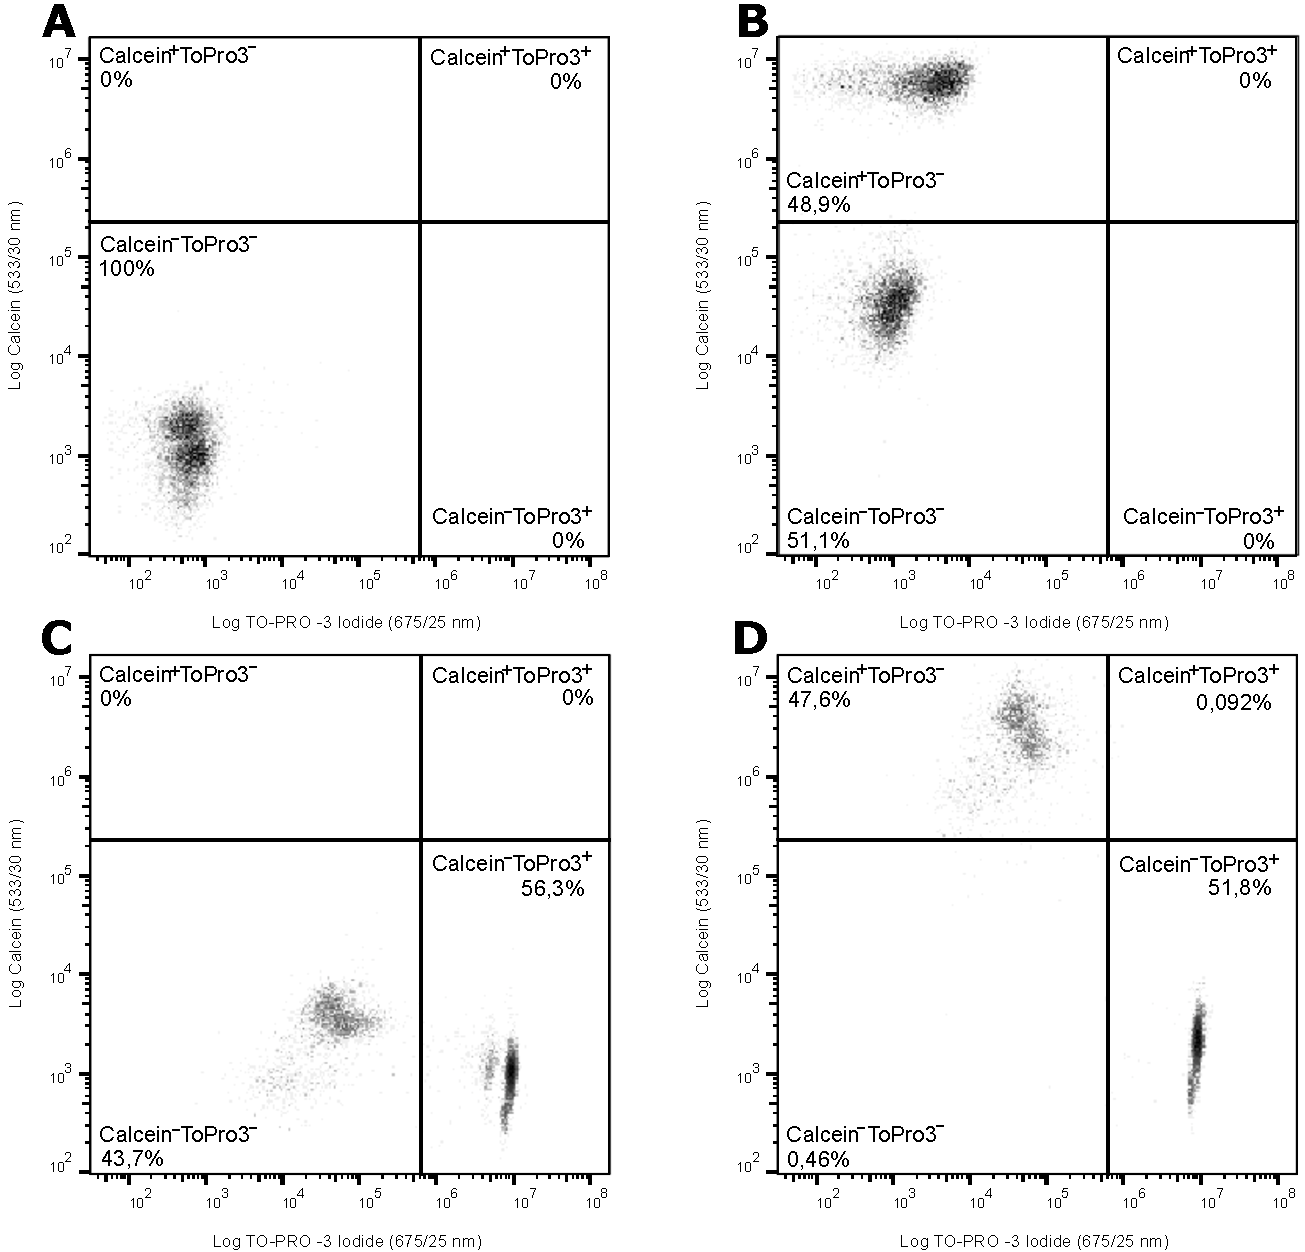
\includegraphics[width=.7\textwidth]{figures/Gating strategy/ToPro3 CAM gating strategy.pdf}
    \caption{\textbf{FL1 (533/30 nm) vs. FL4 (675/25 nm) quadrant gating for flow cytometric scoring of necrotic (Calcein$^{-}$ ToPro3$^{+}$) an viable (Calcein$^{+}$ ToPro3$^{-}$) haemocytes.} By preparing a pool of \ce{MeOH}-killed and newly withdrawn haemocytes in antiaggregative buffer (\acrshort{acb}), gates were drawn according to the florescent profiles of \textbf{A)} Unstained controls, \textbf{B)} Calcein \acrshort{fmo}s, \textbf{C)} TO-PRO$^{TM}$-3 Iodide FMOs and \textbf{D)} aliquotes stained with both probes.}
    \label{fig:TP3_Calcein_gating_strat}
\end{figure}

The unstained controls were used to establish a tentative lower left quadrant gate (Calcein$^{-}$ ToPro3$^{-}$), as seen in Figure \ref{fig:TP3_Calcein_gating_strat}A. This quadrant was expanded in both directions to include all Calcein$^{-}$ events of the Calcein FMOs and all the ToPro3$^{-}$ events of the TO-PRO$^{TM}$-3 Iodide FMOs (see Figure \ref{fig:TP3_Calcein_gating_strat}B and C). When the double stained samples were run, the viable and methanol-killed haemocytes populated the upper left and lower right quadrants, exclusively.

\subsubsection{Method validation}
A flow cytometer is a very sensitive instrumentation for measuring fluorescent signals, and with a throughput of up to 10.000 events s$^{-1}$, these instruments represent a far superior technology for counting fluorescent cells compared to epifluorescent microscopy. However, the result obtained from a flow cytometric assay is entirely dependent on the gating strategy employed to generate the results. An effort was therefore made to cross-validate the gating strategy presented in the previous section by epifluorescent microscopy.

Methanol-killed (70\% \acrshort{meoh}, 30 min) and freshly withdrawn haemocytes (\acrshort{acb}, 1:1) were mixed in semi-random proportions to prepare 10 samples with 0-100\% necrotic haemocytes. Samples were stained with Calcein AM (50 nM) and TO-PRO$^{TM}$-3 Iodide (1.2 \micro M) for 15 minutes, and 10.000 events were acquired from each sample on the BD Accuri C6 Plus flow cytometer. Events were gated according to the strategy presented in Figure \ref{fig:TP3_Calcein_gating_strat}.

\begin{figure}[H]
    \centering
    \begin{subfigure}[b]{.45\textwidth}
        \centering
        \includegraphics[width=\textwidth]{figures/Method development/Cy5 B2A/M7 7 Cy5 cropped.png}
        \caption{TO-PRO$^{TM}$-3 Iodide fluorescence collected from microscopic field with a LED-Cy5-A filter cube.}
        \label{subfig:a}
    \end{subfigure}
    \hfill
    \begin{subfigure}[b]{.45\textwidth}
        \centering
        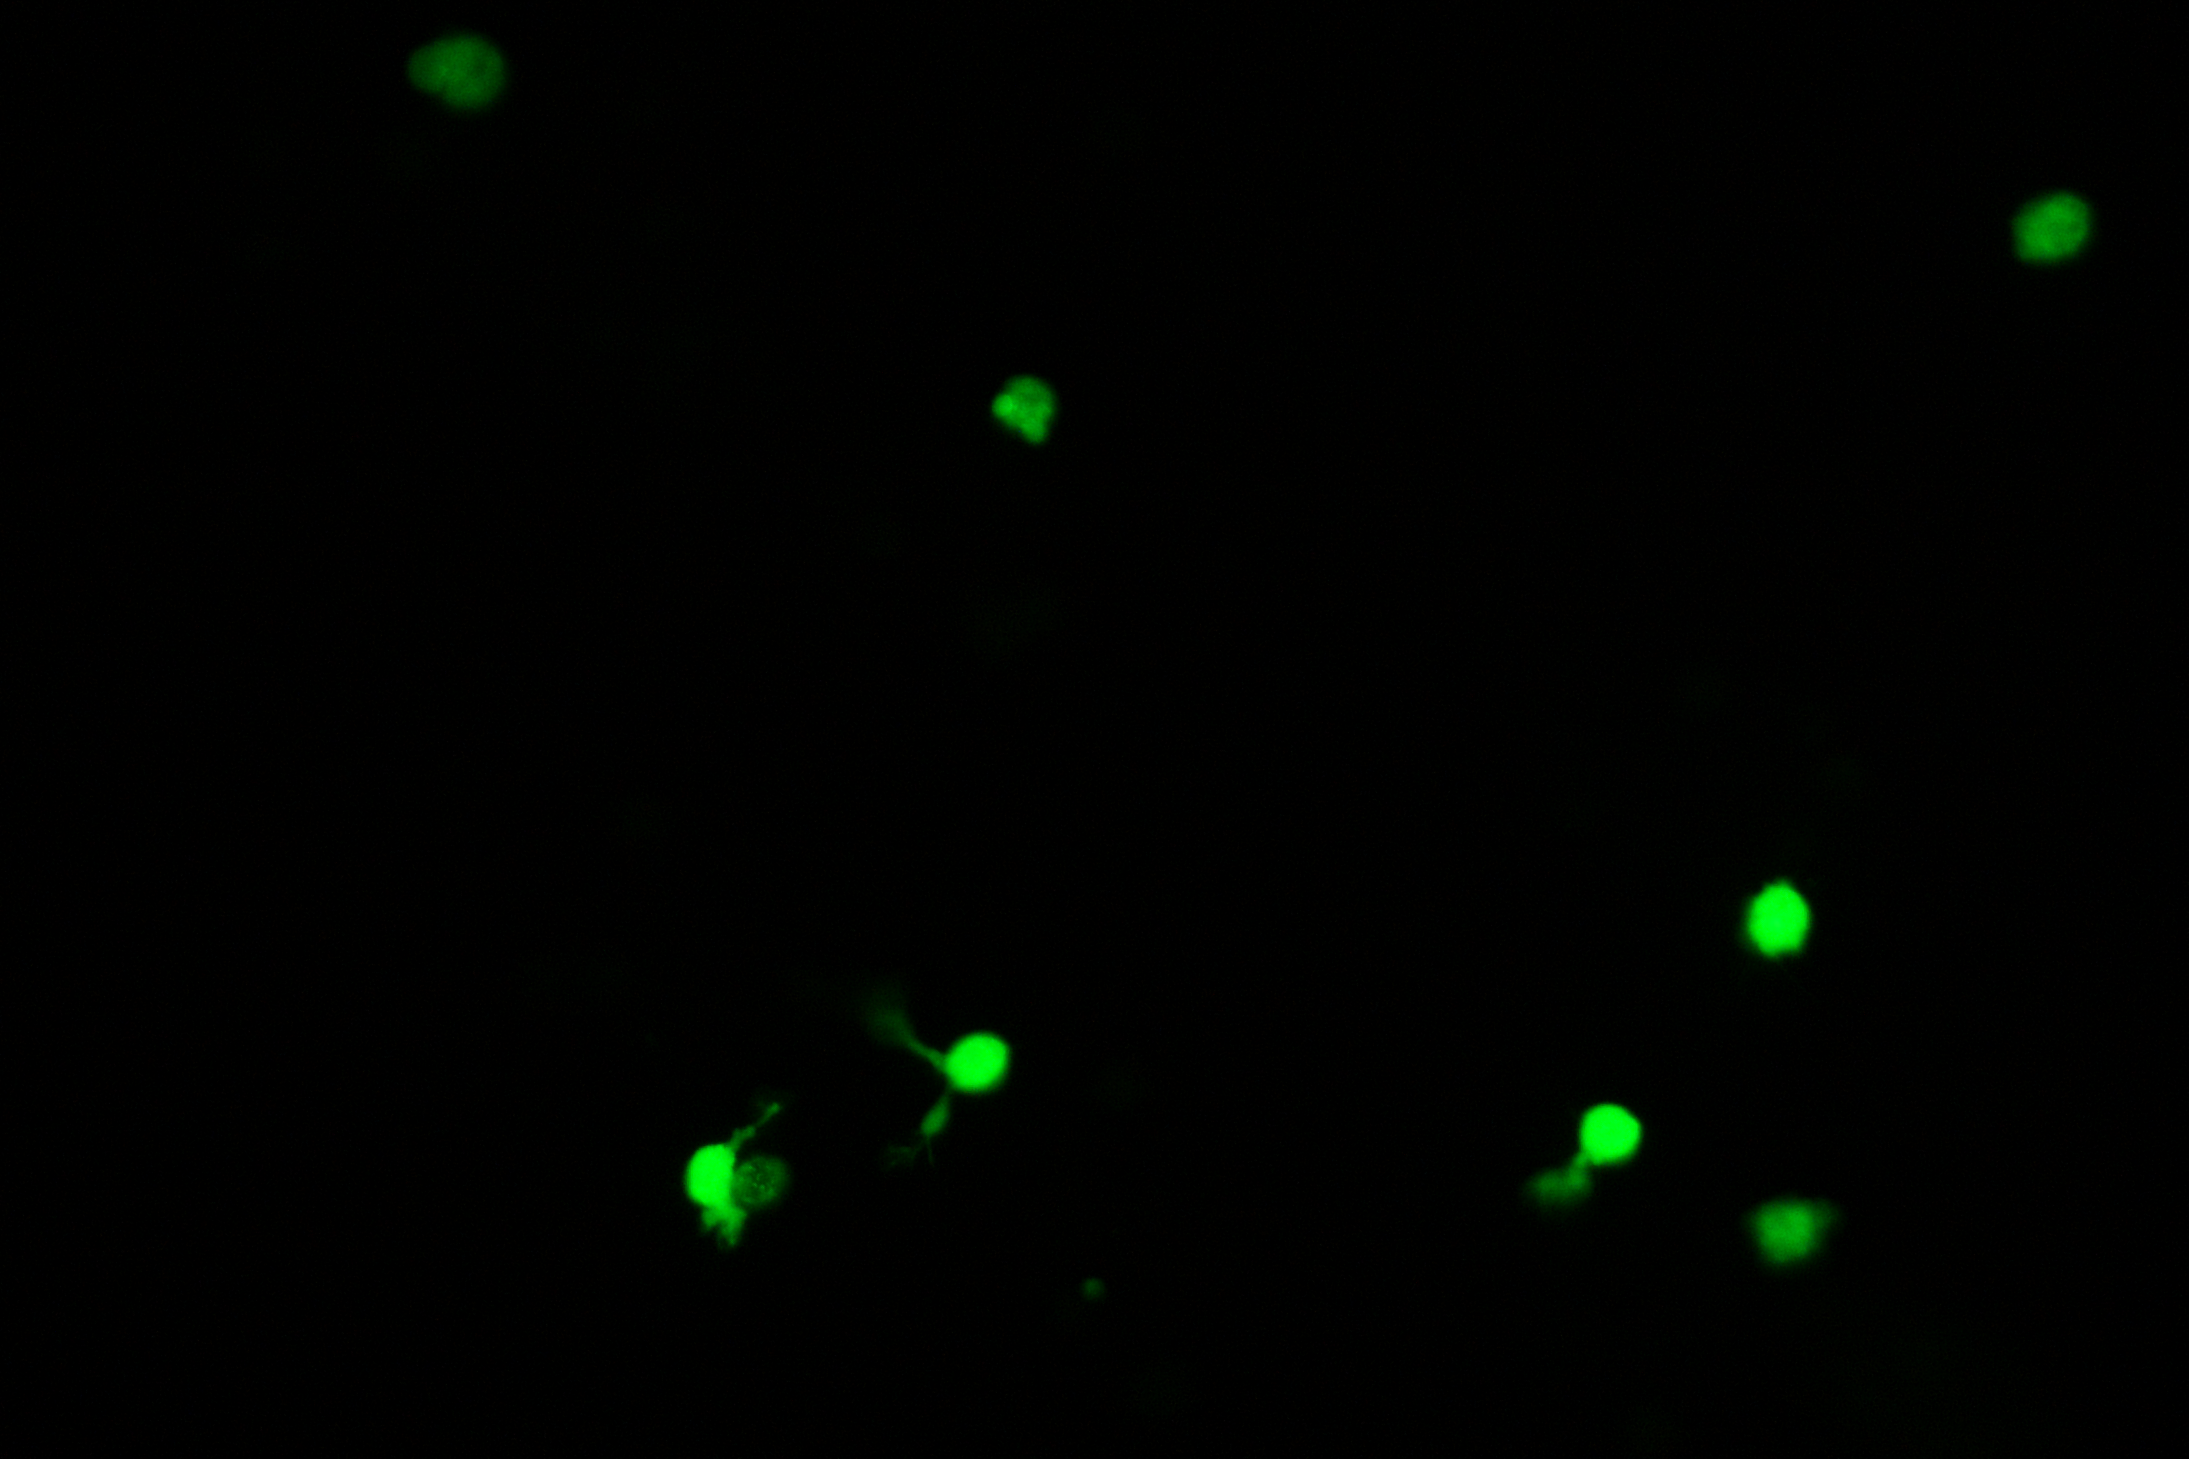
\includegraphics[width=\textwidth]{figures/Method development/Cy5 B2A/M7 7 B2A cropped.png}
        \caption{Calcein fluorescence collected from the same microscopic field with a B-2A filter cube.}
        \label{subfig:b}
    \end{subfigure}
    \newline
    \begin{subfigure}[b]{.45\textwidth}
        \centering
        \includegraphics[width=\textwidth]{figures/Method development/Cy5 B2A/M7 7 DIC cropped.png}
        \caption{Microscopic field imaged by DIC microscopy to verify cellular identities of fluorescent signals.}
        \label{subfig:c}
    \end{subfigure}
    \hfill
    \begin{subfigure}[b]{.45\textwidth}
        \centering
        \includegraphics[width=\textwidth]{figures/Method development/Cy5 B2A/M7 7 Merged cropped.png}
        \caption{Merged RGB image from the red and green color planes of image \emph{a} and \emph{b}, respectively.}
        \label{subfig:d}
    \end{subfigure}
    \caption{An illustration of the image analysis used to score necrotic and viable haemocytes by epifluorescence and DIC microscopy at 20x magnification.}
    \label{fig:Epifluorescent_scoring}
\end{figure}

Following flow cytometric acquisition, the 10 samples were transferred onto glass slides, coverslipped and put on the stage of a Nikon 90i upright microscope equipped with a DS-Fi1c microscope camera (Nikon, Tokyo, JP). Ten microscopic fields were imaged per slide at 20x magnification, and each field was imaged in three subsequent steps (see Figure \ref{fig:Epifluorescent_scoring}): (1) Epifluorescence microscopy with a LED-Cy5-A filter cube, 6 s exposure and 4.8 gain (2) epifluorescent microscopy with a B-2A filter cube, 400 ms exposure and 2.0 gain, followed by (3) DIC microscopy. The red and green color planes of the two epifluorescence images were merged into an RGB image in NIS Elements D (D v.3.22.15) software, and the percentages of necrotic, viable and doubly stained haemocytes were scored using the merged image (see Figure \ref{fig:Epifluorescent_scoring}d). The DIC images were used to confirm the identity of the fluorescent signals, such that only cellular fluorescence was included in the counts.

To examine the correlation between results obtained by flow cytometry and fluorescent microscopy, the percentage of necrotic haemocytes (Calcein$^{-}$ ToPro3$^{+}$) were analyzed by linear regression using the base R \emph{lm} function (\cite{R-project}). The percentage of necrotic haemocytes (\%) were calculated according to (\ref{eq:necrotic hemocytes_2}), such that double positive haemocytes were counted as viable. The imaging process took up to one 1 hour per slide, so any double positive haemocytes had most likely become necrotic during the course of microscopy. It should be noted that samples were prepared and scored one at a time to minimize the occurrence of \emph{in vitro} necrosis.

\begin{equation}
    \label{eq:necrotic hemocytes_2}
    \text{Necrotic haemocytes (\%)} = \dfrac{n_{Calcein^{-}ToPro3^{+}}}{n_{total} - n_{Calcein^{-}ToPro3^{-}}} \times 100
\end{equation}

\section{Method}
\subsection{Animal housing}
Adult blue mussels (\emph{Mytilus edulis}) of x.x$\pm{5}$ cm shell length were obtained from Snadder og Snaskum AS (Indre Fosen, Norway). Upon arrival at the marine animal housing facilities of NTNU, Centre of Fisheries and Aquaculture (SeaLab), the mussels were transferred to 50 L filtered seawater flow-through tanks (11 L/min) supplied by a direct inlet from Trondheimsfjorden at 80 m depth ($\SI{7.5}{\celsius}$). Here, the mussels were kept to acclimatize for 2 days before transfer to the experimental exposure setup.

Time of mussel harvest/purchase?

Describe water treatment in more detail: include information regarding sand-filter, protein-skimmer, 0.5 um filter bags and UV-treatment.

Because the watertreatment left no natural feed for the mussels, the filtered seawater were supplemented with algae [insert species \& frequency].


\subsection{Experimental setup/design}
- Specs related to flowrate, feeding (alge conc: Coulter counter), how often was nano particles changed (every 3-4 days: check article), concentrations (ICP-MS --> mg/L in stocks and exp tanks), zetasizer --> size and surface potential

include figure of exp setup?

depuration period: check article

storage from depuration to sampling: mussels were not kept on ice, but were washed and taken directly upstairs for measuring weight, length, height and width for condition index, and were given to us for \acrshort{fcm} sampling afterwards. If we were delayed, they were kept in the fridge until hemolymph sampling 

\subsection{Hybrid Micronucleus Assay}
Sampling
Flow Cytometer used and Flow Cytometry acquisition software
External software used for graphing and analysis of exported FCS files.
Replicate/triplicate measurements?
Number of events recorded for each mussel?
Briefly describe FCS and \acrshort{ssc}.
Mention if data were collected in linear or logarithmic scale, 
FSC treshold (80.000 FSC-H). 
Fluorescent compensation (matrix)
Describe gating strategy herein? Debris exclusion (size); doublet exclusion --> haemocytes. (Gating of basophils and eosinophils, the use of \acrshort{fmo} controls with TO-PRO-3 and/or the apoptosis stain) to create gates.

\begin{table}[H]
	\centering
	\caption{The \acrshort{fcm} acquisition and fluidics settings specified with the BD Accuri C6 Plus acquisition software during the flow cytometric experiments reported in this work.}
	\label{tb:FCM_settings}
	\resizebox{\linewidth}{!}{
	\begin{tabular}{lllll}
	\textbf{Experiment nr.} & \textbf{Event-triggering threshold} & \textbf{Acquisition stop-condition} & \textbf{Flow rate (\micro L/min)} & \textbf{Core size (\micro m)} \\
		\midrule
    Aggregation & 80.000 FSC-H & acquired volume, 20 \micro L & 30 & 10 \\
    Calcein AM and TO-PRO$^{TM}$-3 Iodide & 80.000 FSC-H & 10.000 haemocyte events & 36 & 16 \\
    Apo-15 and TO-PRO$^{TM}$-3 Iodide & 80.000 FSC-H & 10.000 haemocyte events & 36 & 16 \\
		\bottomrule
	\end{tabular}
	}
\end{table}

\subsubsection{Scoring of necrotic haemocytes}

\subsubsection{Scoring of apoptotic haemocytes}

\subsubsection{Differential haemocyte count}

\subsubsection{Determination of haemocyte concentration}

\subsubsection{Slide preparation}
Refer to the MN cytome assay by Bolognesi, and mention that we fixed and stained haemocytes in suspension to produce slides without aggregated haemocytes. Since the cells were dead, they did not spread or produce pseudopodia, which allowed us to observe the actual size and form which they would posses ass they flowed through the laser of the flow cytometer.

\subsubsection{Scoring of MN and nuclear anomalies}

\subsubsection{Measurements and calculations}
(\cite{R-project})

\subsubsection{Statistical analysis}
